% COMPILE: xelatex

\documentclass[a4paper]{article}  % A4 paper size

\usepackage[UTF8]{ctex}  % Chinese support
\usepackage[left=3.17cm, right=3.17cm, top=2.54cm, bottom=2.54cm]{geometry}  % Margins

\usepackage{xcolor}  % Color support
\usepackage{tcolorbox}  % Colored boxes

\usepackage{fancyhdr}  % Header and footer
\usepackage{graphicx, subcaption}  % Figures
\usepackage[shortlabels]{enumitem}  % Enumerate list
\usepackage[sort&compress]{gbt7714}  % Bibliography
\usepackage{hyperref}  % Hyperlinks
\usepackage{booktabs, array}  % Tables
\usepackage{multirow}  % Multirow
\usepackage{amsmath}  % Math

\tcbuselibrary{skins}  % Colored boxes
\tcbuselibrary{minted}  % Code blocks
\tcbuselibrary{breakable} % Allow page breaks in code blocks

\setmonofont[]{Fira Code}  % Monospaced font
\usemintedstyle{colorful}  % Code block style set up
\setenumerate{  % Enumerate list set up
    itemsep=0pt,
    partopsep=0pt,
    parsep=\parskip,
    topsep=0pt,
    itemindent=4em,
    leftmargin=0pt,
    listparindent=2em,
    label= (\arabic*)
}
\setitemize{  % Itemize list set up
    itemsep=0pt,
    partopsep=0pt,
    parsep=\parskip,
    topsep=5pt
}
\setdescription{  % Description list set up
    itemsep=0pt,
    partopsep=0pt,
    parsep=\parskip,
    topsep=5pt
}
\hypersetup{  % Hyperlinks set up
    unicode,
    colorlinks=true,
    linkcolor=black,
    urlcolor=black
}



\newtcblisting{codeblock}[2][]{
    listing engine=minted,
    boxrule=0.1mm,
    colback=white!98!black,
    colframe=white!80!black,
    listing only,
    left=5mm,
    enhanced,
    sharp corners=all,
    breakable,
    overlay={
        \begin{tcbclipinterior}
            \fill[white!98!black] (frame.south west) rectangle ([xshift=5mm]frame.north west);
        \end{tcbclipinterior}
    },
    minted language=#2,
    minted style=tango,
    minted options={fontsize=\small,breaklines,autogobble,linenos,numbersep=3mm,escapeinside=\#\#},#1  % Use \# as escape character
}


\begin{document}

\title{\textbf{通信原理实验报告}}
\author{纳姆露丝}
\date{\today}
\maketitle

\tableofcontents

\newpage

\begin{abstract}
    ABSTRACT
\end{abstract}

\section{实验设计}

本实验系统由四个主要模块组成:Hamming 编解码、交织与解交织、QPSK 调制解调以及加性高斯白噪声(AWGN)信道。这些模块协同工作,模拟实际通信系统中的信号处理与传输过程。

\subsection{Hamming 编解码}



\subsection{交织与解交织}



\subsection{QPSK 调制解调}

在现代数字通信系统中,QPSK(Quadrature Phase Shift Keying,正交相位调制)是一种高效的调制方式,它通过在同一时间内传输两个比特来实现高数据传输率。如图 \ref{fig:qpsk_model} 所示,QPSK 调制器将输入的二进制数据分成两部分,每部分表示一个信号的相位,分别控制正交的两个载波(I路和Q路)。这种方式可以有效利用带宽,同时保持较高的抗干扰能力。

\begin{figure}[ht]
    \centering
    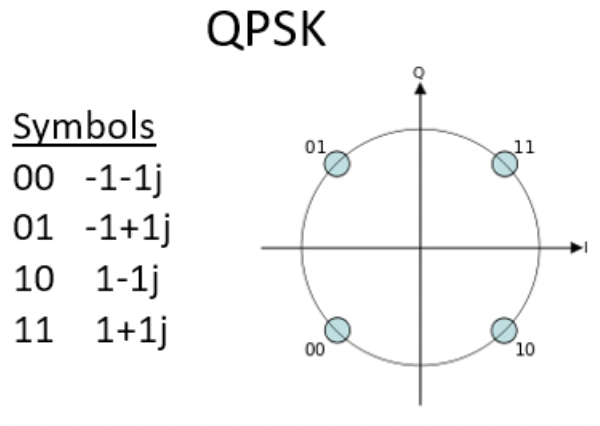
\includegraphics[width=.3\textwidth]{static/qpsk_model.png}
    \caption{QPSK 调制解调模型}
    \label{fig:qpsk_model}
\end{figure}

QPSK 调制与解调过程包括以下几个步骤:

\begin{itemize} 
    \item 调制过程:输入的数据每两位作为一个信号符号,映射到四个不同的相位上,通常是 $0^\circ$,$90^\circ$,$180^\circ$ 和 $270^\circ$,分别对应不同的比特组合。
    \item 解调过程:接收端根据信号的相位变化来恢复发送的比特流。通过比较接收到的信号与阈值,判断其属于哪个相位,并输出对应的比特组合。
\end{itemize}





\subsection{AWGN 信道模型}

AWGN(Additive White Gaussian Noise,加性白噪声)信道模型广泛应用于无线通信领域,用于模拟理想情况下的噪声影响。在此信道模型中,噪声是加性、均匀分布的,且具有高斯分布特性。在本实验中,AWGN 信道的模拟过程分为两个步骤:首先,通过 LFSR(线性反馈移位寄存器)生成伪随机数序列;然后,利用 Box-Muller 变换将这些伪随机数转换为服从高斯分布的随机数,最终将这些噪声加到信号中,模拟实际通信中的噪声干扰。

\subsubsection{LFSR}

为了产生 Gaussian 白噪声,首先需要生成均匀分布的伪随机数序列。本实验中,我们采用线性反馈移位寄存器(LFSR),通过移位寄存器和特定的反馈函数来生成这些随机数。

图 \ref{fig:lfsr_model} 展示了一个 16 位 Fibonacci LFSR。其采用的特征多项式为 $X^{16} + X^{14} + X^{13} + X^{11} + 1$。该多项式确保了生成的随机序列的周期最大(65535,不包括全零状态),以有效地模拟随机性。移位寄存器逐位输出随机序列的每一位,同时通过反馈机制决定下一个状态。这一过程不断重复,直到达到最大周期。例如,图中的状态为 0xACE1 (十六进制) ,下一个状态是 0x5670.

\begin{figure}[ht]
    \centering
    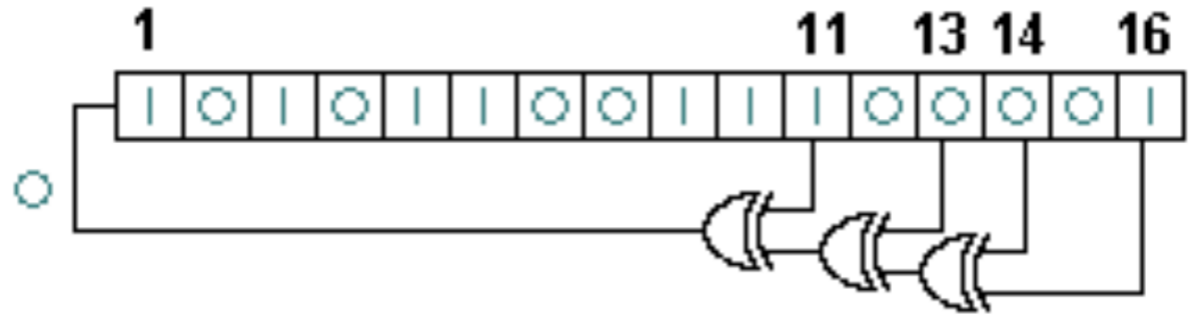
\includegraphics[width=.6\textwidth]{static/lfsr_model.png}
    \caption{一个 16-位 Fibonacci LFSR}
    \label{fig:lfsr_model}
\end{figure}

\subsubsection{Box-Muller}

Box-Muller 变换是一种用于从均匀分布的随机数生成高斯分布随机数的方法。在本实验中,我们首先生成两个均匀分布的随机数 $U_1, U_2 \sim U(0, 1)$,然后通过以下公式将其转换为符合标准正态分布的随机数:

$$
\begin{aligned}
X = \sqrt{-2\ln U_1} \cos(2\pi U_2) \\
Y = \sqrt{-2\ln U_1} \sin(2\pi U_2)
\end{aligned}
$$

其中,$X$ 和 $Y$ 分别为符合标准正态分布的随机变量。


\section{实验过程}

\subsection{Hamming 编解码}



\subsection{交织与解交织}



\subsection{QPSK 调制解调}

QPSK 调制器:

\begin{itemize} 
    \item QPSK 调制器根据输入的 2 比特数据,将其分别映射为 I 路和 Q 路的符号。
    \item 由于 QPSK 调制是基于正交载波的,调制器的输出信号对应于一个复数的实部和虚部,分别通过 I 路和 Q 路输出。
    \item 具体实现中,我们通过将每个输入符号映射到 ±1/√2 乘以常数值来实现 QPSK 调制。常数值为 $1/\sqrt{2}$,其作用是对输出信号进行归一化处理,避免过强的信号造成干扰。
\end{itemize}

Verilog 关键代码如下:

\begin{codeblock}{verilog}
localparam signed [15:0] CONST_VAL = 16'b0101_1011;  // 1/sqrt(2)
always @(posedge clk or negedge rst) begin
    if (~rst) begin
        data_o_i <= 16'b0;  data_o_q <= 16'b0;
    end else begin
        case (data_i)
            2'b00: begin
                data_o_i <= CONST_VAL;  data_o_q <= CONST_VAL;
            end
            2'b01: begin
                data_o_i <= -CONST_VAL; data_o_q <= CONST_VAL;
            end
            2'b10: begin
                data_o_i <= CONST_VAL;  data_o_q <= -CONST_VAL;
            end
            2'b11: begin
                data_o_i <= -CONST_VAL; data_o_q <= -CONST_VAL;
            end
            default: begin
                data_o_i <= 16'b0;      data_o_q <= 16'b0;
            end
        endcase
    end
end
\end{codeblock}

QPSK 解调器:

\begin{itemize} 
    \item 解调器的作用是根据接收到的 I 路和 Q 路信号,判断信号属于哪一个象限,进而恢复原始数据。
    \item 解调器通过比较 I 路和 Q 路信号与阈值的大小关系,来判断比特的值。阈值设置为零,即信号大于零则为 1,小于零则为 0。
\end{itemize}

Verilog 关键代码如下:

\begin{codeblock}{verilog}
localparam signed [15:0] THRESHOLD = 16'b0;
always @(posedge clk or negedge rst) begin
    if (~rst) begin
        data_o <= 2'b00;
    end else begin
        if (data_i_i > THRESHOLD) begin
            if (data_i_q > THRESHOLD)   data_o <= 2'b00;
            else                        data_o <= 2'b10;
        end else begin
            if (data_i_q > THRESHOLD)   data_o <= 2'b01;
            else                        data_o <= 2'b11;
        end
    end
end
\end{codeblock}





\subsection{AWGN 信道模型}

\subsubsection{LFSR 生成均匀分布随机数}

在本实验中,为保证生成的两组随机数序列的独立性,LFSR 的伪随机数序列通过不同的特征多项式、不同的种子生成。具体地,选用不同的 SEED 值(即种子),并根据其最低有效位(LSB)选择特定的反馈多项式:

\begin{itemize} 
    \item SEED[0] = 1 时,特征多项式为 $X^{16} + X^{14} + X^{13} + X^{11} + 1$ 
    \item SEED[0] = 0 时,特征多项式为 $X^{16} + X^{15} + X^{13} + X^{4} + 1$ 
\end{itemize}

Verilog 代码实现如下:

\begin{codeblock}{verilog}
reg [15:0] lfsr_state;

always @(posedge clk or posedge rst) begin
    if (rst) begin
        lfsr_state <= SEED;
    end else begin
        if (SEED[0] == 1) begin
            lfsr_state <= {lfsr_state[14:0], lfsr_state[15] ^ lfsr_state[13] ^ lfsr_state[12] ^ lfsr_state[10]};
        end else begin
            lfsr_state <= {lfsr_state[14:0], lfsr_state[15] ^ lfsr_state[14] ^ lfsr_state[12] ^ lfsr_state[3]};
        end
    end
end
\end{codeblock}

在此过程中,生成的伪随机数序列被用于模拟 AWGN 信道中的噪声影响。为了确保生成的随机数适应特定范围的需求,采用如下代码进行范围调整:

\begin{codeblock}{verilog}
assign uniform_o = lfsr_state % (O_MAX - O_MIN + 1'b1) + O_MIN;
\end{codeblock}

该过程通过调整输出值的范围,确保生成的随机数序列符合信道噪声的要求。


\subsubsection{Box-Muller 生成高斯分布随机数}

为了提高系统的效率,我们采用查表法来计算 Box-Muller 变换中的 $\ln U_1$ 以及 $\cos(2 \pi U_2)$,以减少计算复杂度。具体来说,我们通过查表将 $U_1$ 和 $U_2$ 映射到预先计算好的值,从而实现快速变换。

特别地,对于 $\cos(2 \pi U_2)$,我们利用对称性和奇偶性,仅对 $U_1 \in [0, 0.25]$ 的部分进行查表映射,从而降低了存储需求并提高了查表效率:

\begin{codeblock}{verilog}
    wire cos_sign;
    assign cos_sign = (uniform_o_0 <= 256) ? 0 :
                      (uniform_o_0 <= 768) ? 1 :
                      0;
    wire [15:0] cos_addr;
    assign cos_addr = (uniform_o_0 <= 256) ? (uniform_o_0 - 1) :
                      (uniform_o_0 <= 512) ? (512 - uniform_o_0) :
                      (uniform_o_0 <= 768) ? (uniform_o_0 - 513) :
                      (1024 - uniform_o_0);
    wire signed [7:0] cos_lut_o;
    cos_lut cos_lut_0 (
        .addr(cos_addr),
        .cos_out(cos_lut_o)
    );

    wire signed [7:0] cos_o;
    assign cos_o = cos_sign ? -cos_lut_o : cos_lut_o;
\end{codeblock}

为了有效处理计算和存储,Box-Muller 变换的实现采用了定点数表示,通过算术左移和右移操作,在不溢出的情况下平衡了计算精度和速度。


\section{仿真测试}

本次实验使用 Vivado 2017.3 进行仿真测试。

\subsection{Hamming 编解码}

仿真文件如下:
\begin{codeblock}{verilog}
`define PERIOD 10
module hamming_tb();
    reg [3:0] data_i;
    wire [6:0] data_enc;
    wire [3:0] data_dec;
    hamming_encode hamming_encode_0 (
        .data_i(data_i),
        .data_o(data_enc)
    );
    hamming_decode hamming_decode_0 (
        .data_i(data_enc),
        .data_o(data_dec)
    );
    integer i;
    initial begin
        for (i = 0; i < 16; i=i+1) begin
            data_i = i;
            #(`PERIOD)
            if (data_dec ! = data_i) begin
                $display("[Error]: %b -> %b -> %b", data_i, data_enc, data_dec);
            end 
            else begin
                $display("Correct: %b -> %b -> %b", data_i, data_enc, data_dec);
            end
        end
    end
endmodule
\end{codeblock}

输出如下:
\begin{codeblock}{verilog}
Correct: 0000 -> 0000000 -> 0000
Correct: 0001 -> 1110001 -> 0001
Correct: 0010 -> 1010010 -> 0010
Correct: 0011 -> 0100011 -> 0011
Correct: 0100 -> 0110100 -> 0100
Correct: 0101 -> 1000101 -> 0101
Correct: 0110 -> 1100110 -> 0110
Correct: 0111 -> 0010111 -> 0111
Correct: 1000 -> 1101000 -> 1000
Correct: 1001 -> 0011001 -> 1001
Correct: 1010 -> 0111010 -> 1010
Correct: 1011 -> 1001011 -> 1011
Correct: 1100 -> 1011100 -> 1100
Correct: 1101 -> 0101101 -> 1101
Correct: 1110 -> 0001110 -> 1110
Correct: 1111 -> 1111111 -> 1111
\end{codeblock}

这表明 Hamming 码编解码模块实现正确。

\subsection{交织与解交织}

仿真文件如下:
\begin{codeblock}{verilog}
module test_IL();  
    reg clk;
    reg rst;
    reg en;
    reg [28 -1:0] data = 28'b0011111000011110110111100101;
    wire en_IL;
    wire [28 -1:0] data_IL;
    interleaver il(clk, rst, en, data, en_IL, data_IL);
    wire [28 -1:0] data_DIL;
    wire en_DIL;
    deinterleaver dil(clk, rst, en_IL, data_IL, en_DIL, data_DIL);
    initial begin
        clk <= 1;
        rst <= 0;
        en <= 0;
        #10 en <= 1;
        rst <= 1;
    end
    always #5 clk = ~clk; 
endmodule
\end{codeblock}

仿真结果如图 \ref{fig:interleave_simulation1} 所示。

\begin{figure}[ht]
    \centering
    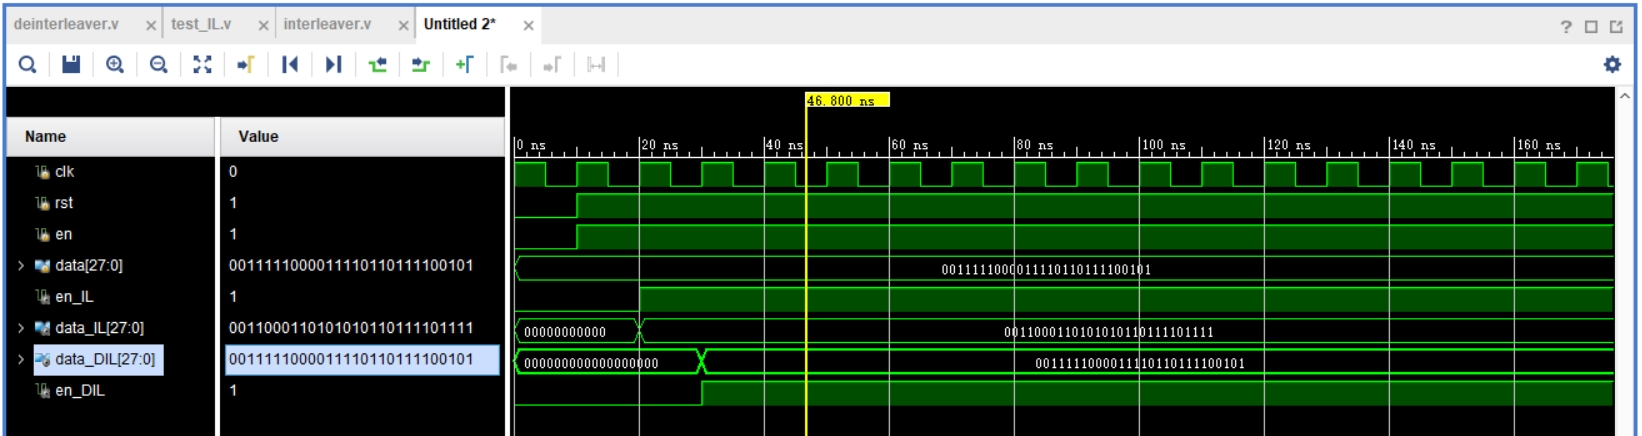
\includegraphics[width=1.0\textwidth]{static/interleave.png}
    \caption{交织与解交织仿真波形}
    \label{fig:interleave_simulation1}
\end{figure}

如图 \ref{fig:interleave_simulation2} 所示,按照“按行写入,按列读出”这一规则处理输入序列 0011111 0000111 1011011 1100101,得到的交织器输出序列应为 0011000 1101010 1011011 1101111,与图 \ref{fig:interleave_simulation1} 中的data\_IL 波形一致,说明交织器设计正确,且data\_DIL 和输入序列 data 相同,说明解交织器设计正确。

\begin{figure}[ht]
    \centering
    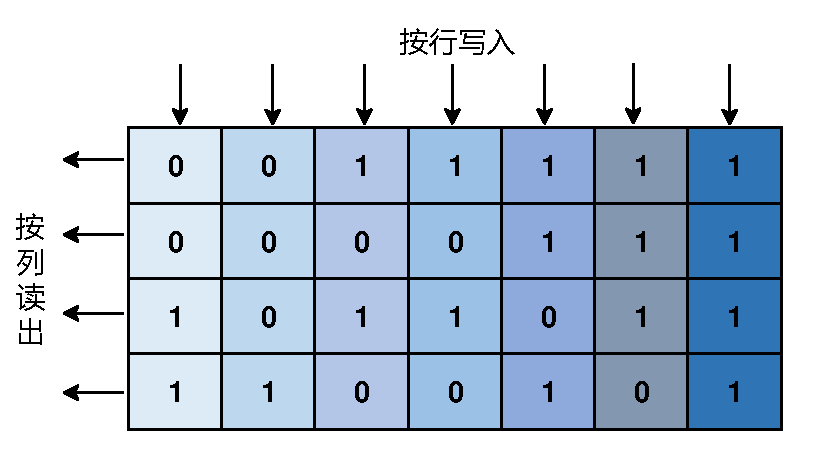
\includegraphics[width=.7\textwidth]{static/interleave_simulation.pdf}
    \caption{交织过程演示}
    \label{fig:interleave_simulation2}
\end{figure}

\subsection{QPSK 调制解调}

仿真文件如下:
\begin{codeblock}{verilog}
module test();
    parameter clk_period_100M = 10; // f=100MHz <=> T=10ns
    reg rst;
    reg clk;
    reg [15:0] datas = 16'b1110110110001101;
    wire [1:0] data_i;
    assign data_i = datas[1:0];
    wire signed [15:0] data_o_i;
    wire signed [15:0] data_o_q;
    qpsk_modulator qpsk_modulator_0 (
        .clk(clk),
        .rst(rst),
        .data_i(data_i),
        .data_o_i(data_o_i),
        .data_o_q(data_o_q)
    );
    wire [1:0] data_o;
    qpsk_demodulator qpsk_demodulator_0 (
        .clk(clk),
        .rst(rst),
        .data_i_i(data_o_i),
        .data_i_q(data_o_q),
        .data_o(data_o)
    );
    initial begin
        rst <= 0;
        clk <= 1;
        #(clk_period_100M) rst <= 1;
        #(clk_period_100M/2)
        while (datas > 0) begin
            datas <= datas >> 2;
            #(clk_period_100M) ;
        end
    end
    always #(clk_period_100M/2) clk <= ~clk;
endmodule
\end{codeblock}

仿真结果如图 \ref{fig:qpsk_simulation} 所示。

\begin{figure}[ht]
    \centering
    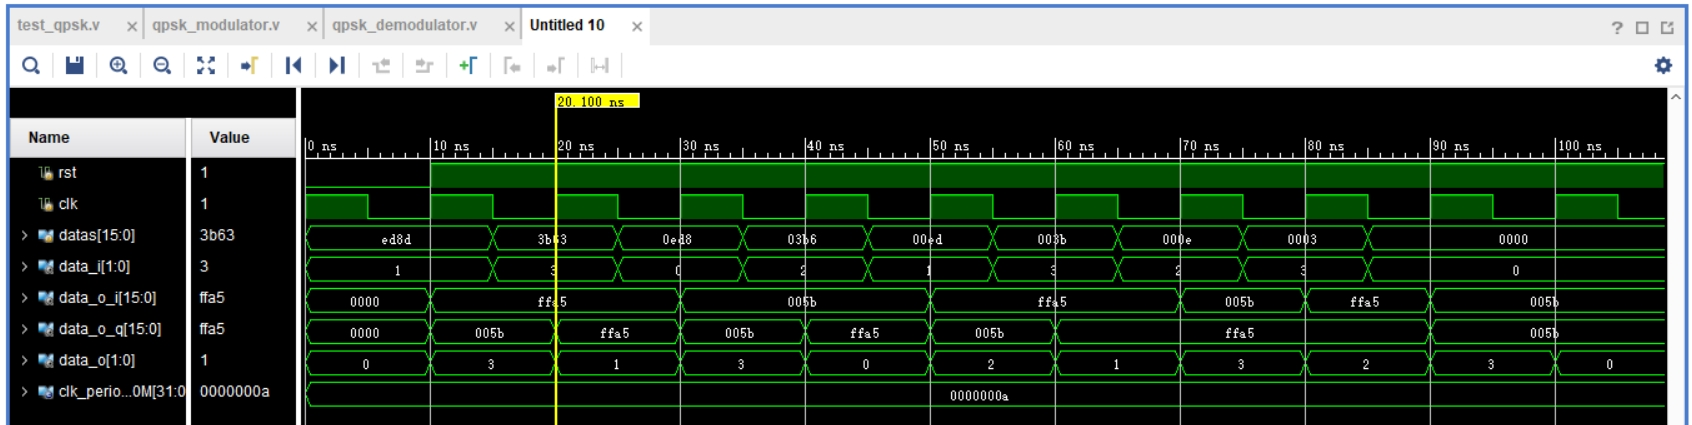
\includegraphics[width=1.0\textwidth]{static/qpsk.png}
    \caption{QPSK 调制解调器仿真波形}
    \label{fig:qpsk_simulation}
\end{figure}

从第三个时钟周期开始,每个时钟周期的 QPSK 解调器的输出 data\_o 都与前一个时钟周期的 QPSK 调制器的输入 data\_i 相等,这说明 QPSK 调制/解调器的设计正确。

\subsection{AWGN 信道模型}

我们保存了仿真产生的高斯白噪声数值,并进行了正态分布假设检验

\begin{codeblock}{verilog}
integer log_file;
initial log_file = \$fopen("simulation_log.txt", "w");
always @(posedge clk) begin
    \$fwrite(log_file, "%d\n", gaussian_noise_channel_0.gaussian_o_0);
    \$fflush(log_file);
end
\end{codeblock}

得到高斯白噪声序列(1000 条),并进行正态分布检验,结果如图 \ref{fig:gaussian_simulation} 所示。可见,概率密度分布和 QQ 图均符合高斯分布的特性。


下面进行严格的正态性检验:

首先进行 Shapiro-Wilk 正态性检验,得到统计量 $W = 0.998$,$p = 0.310$,因此我们无法拒绝高斯分布的假设;同时进行 Kolmogorov-Smirnov 正态性检验,得到统计量 $D = 0.027$,$p = 0.462$,同样无法拒绝高斯分布的假设。

\begin{figure}[ht]
    \centering
    \begin{subfigure}[b]{0.48\textwidth}
        \centering
        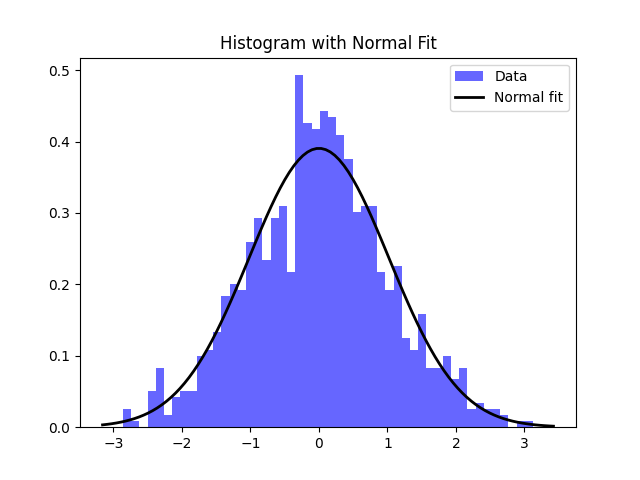
\includegraphics[width=\textwidth]{static/gaussian_fit.png}
        \caption{
            高斯白噪声概率密度分布可视化
        }\label{fig:gaussian_fit}
    \end{subfigure}
    \hfill
    \begin{subfigure}[b]{0.48\textwidth}
        \centering
        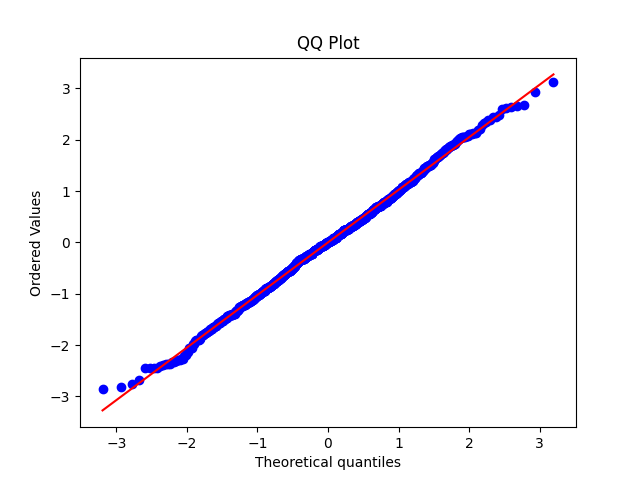
\includegraphics[width=\textwidth]{static/gaussian_qq.png}
        \caption{
            高斯白噪声 QQ 图
        }\label{fig:gaussian_qq}
    \end{subfigure}
    \caption{
        高斯白噪声分布检验
    }\label{fig:gaussian_simulation}
\end{figure}

最后检验自相关性,如图 \ref{fig:gaussian_acf} 所示,分别取 lag 为 20 和 40,自相关性函数均在 0 附近波动,且绝大部分位于 95\% 置信区间内,因此我们可以认为噪声序列是独立同分布的。


\begin{figure}[ht]
    \centering
    \begin{subfigure}[b]{0.48\textwidth}
        \centering
        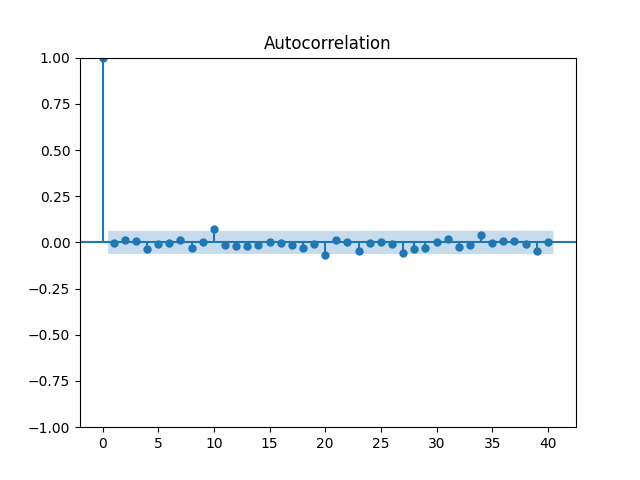
\includegraphics[width=\textwidth]{static/gaussian_acf_40.png}
        \caption{
            高斯白噪声 ACF(lag=40)
        }\label{fig:gaussian_acf_40}
    \end{subfigure}
    \hfill
    \begin{subfigure}[b]{0.48\textwidth}
        \centering
        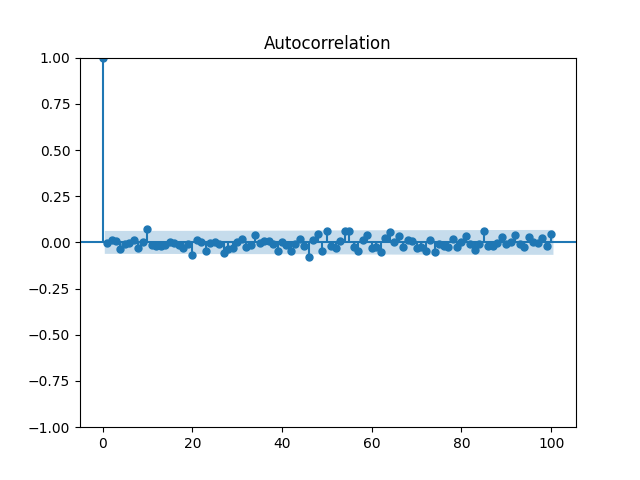
\includegraphics[width=\textwidth]{static/gaussian_acf_100.png}
        \caption{
            高斯白噪声 ACF(lag=100)
        }\label{fig:gaussian_acf_100}
    \end{subfigure}
    \caption{
        高斯白噪声自相关性检验
    }\label{fig:gaussian_acf}
\end{figure}

\subsection{联合仿真}
仿真文件如下:
\begin{codeblock}{verilog}
module test_top();
    reg clk_origin;
    reg rst;
    reg [15:0] button;
    wire [15:0] hamming_dec;
    wire hamming_wave;
    wire interres_wave;
    initial begin
        clk_origin <= 1;
        button <= 16'b0001_0100_0111_1100;
        rst <= 0;
        #5
        rst <= 1;
    end
    always #10 clk_origin = ~clk_origin;
    top top_0 (
        .clk_origin(clk_origin),
        .rst(rst),
        .button(button),
        .hamming_dec(hamming_dec),
        .hamming_wave(hamming_wave),
        .interres_wave(interres_wave)
    );
endmodule
\end{codeblock}

仿真结果如图 \ref{fig:top_simulation1} 所示。

\begin{figure}[ht]
    \centering
    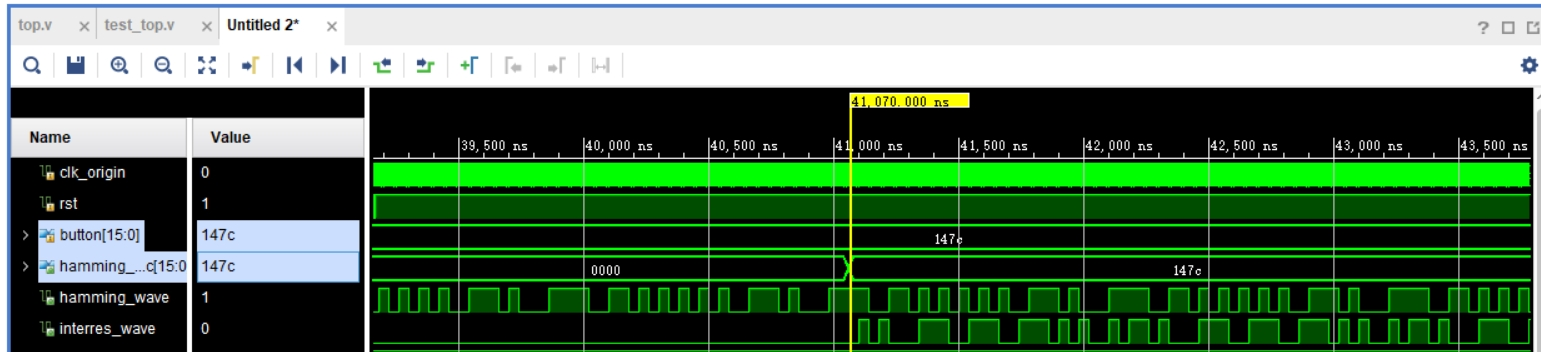
\includegraphics[width=1.0\textwidth]{static/top1.png}
    \caption{联合仿真波形}
    \label{fig:top_simulation1}
\end{figure}

读图可知,系统最终的输出 hamming\_dec 与输入 button 一致,说明系统实现正确。

\section{实验效果}

\section{实验心得}

\section{成员分工}

Hamming 编码、解码:向明义 \\
交织、解交织:游笑权 \\
QPSK 调制解调、AWGN 信道:陈子熠

% % TEXT
% PLAIN
% \textbf{BOLD}
% \textit{ITALIC}
% \underline{UNDERLINE}
% \textcolor{red}{RED}
% \href{https://www.eesast.com}{HYPERLINK}

% % REFERENCE
% ref to section\ref{sec:LABEL}
% ref to figure\ref{fig:LABEL}
% ref to table\ref{tab:LABEL}
% ref to appendix\ref{adx:ASM}
% ref to citation\cite{REF}

% % FIGURE
% \begin{figure}[ht]  % h: here, t: top, b: bottom, p: page
%     \centering
%     \includegraphics[width=.8\textwidth]{FIG.png}  % Width: 0.8 times of text width
%     \caption{CAPTION}\label{fig:FIGURE}
% \end{figure}

% % SUBFIGURE
% \begin{figure}[ht]
%     \centering
%     \begin{subfigure}[b]{0.48\textwidth}
%         \centering
%         \includegraphics[width=\textwidth]{FIG1.png}
%         \caption{
%             CAPTION1
%         }\label{fig:FIG1}
%     \end{subfigure}
%     \hfill
%     \begin{subfigure}[b]{0.48\textwidth}
%         \centering
%         \includegraphics[width=\textwidth]{FIG2.png}
%         \caption{
%             CAPTION2
%         }\label{fig:FIG2}
%     \end{subfigure}
%     \caption{
%         CAPTION1 \\
%         CAPTION2
%     }\label{fig:SUBFIGURE}
% \end{figure}

% % TABLE
% \begin{table}[htb]
%     \centering
%     \caption{CAPTION}\label{tab:LABEL}
%     \begin{tabular}{cc}  % c: center, l: left, r: right, p{2cm}: fixed width
%         \toprule
%         \textbf{HEADER1} & \textbf{HEADER2} \\
%         \midrule
%         CELL1 & CELL2 \\
%         CELL3 & CELL4 \\
%         CELL5 & CELL6 \\
%         \bottomrule
%     \end{tabular}
% \end{table}

% % CODE BLOCK
% \begin{codeblock}{ASM}
%     lw $v0, 114514($sp)
% \end{codeblock}

% % Enumerate list
% \begin{enumerate}[1]  % start from 1
%     % 1: Arabic number, a: Lowercase letter, A: Uppercase letter, i: Lowercase Roman numeral, I: Uppercase Roman numeral
%     \item ITEM1
%     \item ITEM2
%     \item ITEM3
% \end{enumerate}

% % Unreferenced literature
% \nocite{REF}
% \small{
%     \bibliographystyle{gbt7714-numerical}  % gbt7714-plain, gbt7714-numerical
%     \bibliography{ref}  % ref.bib
% }

% \newpage

% % Appendix
% \appendix
% \section{APPENDIX\label{adx:ASM}}


\end{document}